\documentclass[11pt,a4paper]{article}
\usepackage[margin=25mm]{geometry}
\usepackage{booktabs}
\usepackage{graphicx}
\usepackage{hyperref}
\hypersetup{colorlinks=true,urlcolor=blue,linkcolor=blue}
\title{QAOA ACE Golden Study}
\author{BTP / MARS Lab}
\date{26 October 2026}
\begin{document}
\maketitle
\section{Scope and completion contract}
This report is generated only from the dated QAOA study root. The study uses T-HQA placement, mapping seeds 42/43/44, mesh XY/YX/shortest-reliable/maximum-reliability, torus Dijkstra, total memories 2/3/4/6/8/16/32, every legal compiler allocation, ODG/CGP/ACGP/Dynamic full-chain/Dynamic first-hop, and physics seeds 0/1. Primary latency is arrival-to-completion with no historical 5.3-ms subtraction.
\begin{table}[h] \centering \caption{Validated artifact coverage.} \begin{tabular}{lr} \toprule Artifact & Coverage \\\midrule
Base jobs & 1639 / 1639 \\
Policy-seed evaluations & 6402 / 6402 \\
Dynamic auxiliary variant jobs & 143 / 143 \\
Congestion heatmaps & 210 / 210 \\
Mapping route aliases & 15 conceptual / 11 distinct traces \\
\bottomrule \end{tabular} \end{table}
\section{Reproducible data links}
The complete base CSV is available at \href{run:../summaries/base-evaluation-progress.csv}{base-evaluation-progress.csv}. The execution manifest is \href{run:../manifests/base-evaluation_jobs.jsonl.gz}{base-evaluation\_jobs.jsonl.gz} and the congestion summary is \href{run:../congestion/trace_congestion_summary.csv}{trace\_congestion\_summary.csv}.
\section{Congestion heatmap evidence}
\begin{figure}[h] \centering 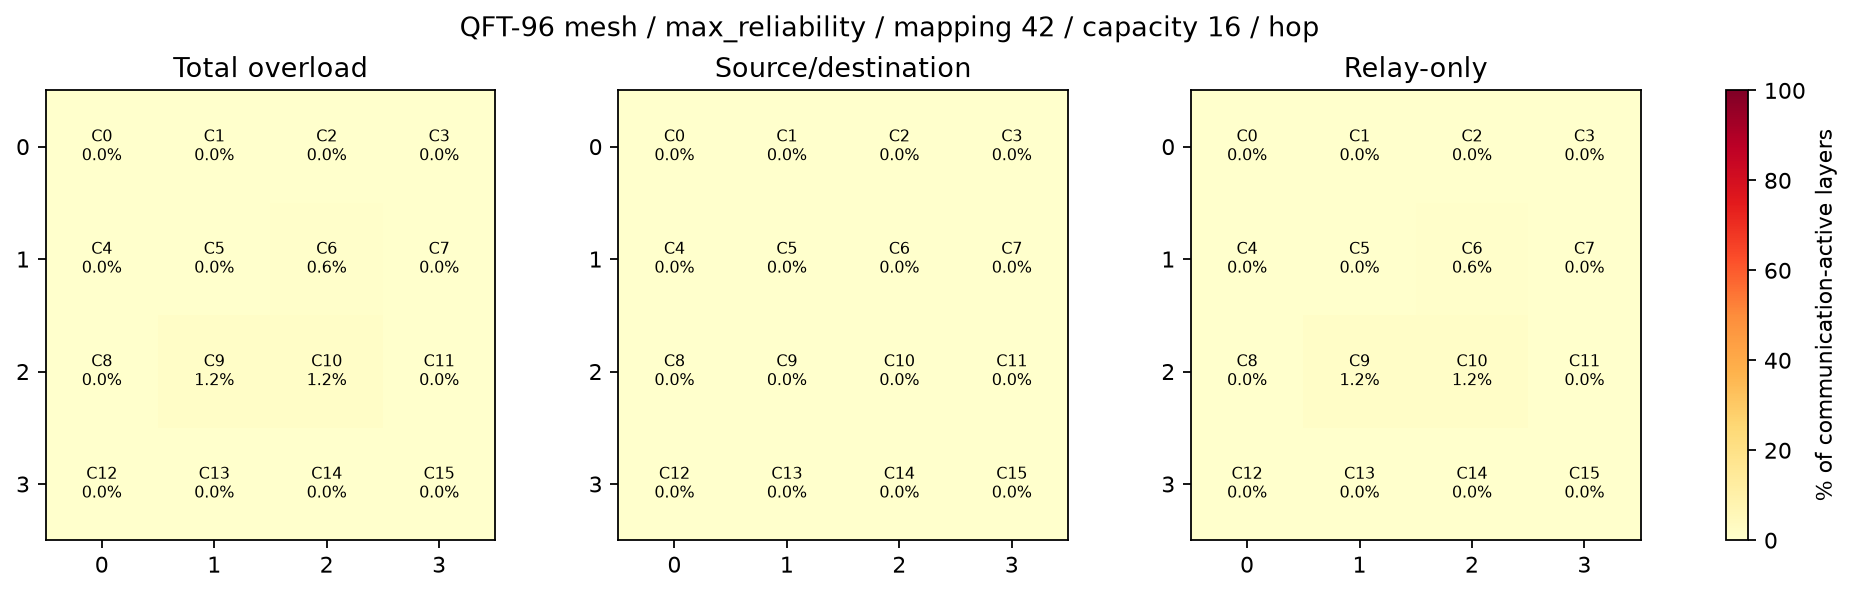
\includegraphics[width=0.98\linewidth]{../congestion/heatmaps/mesh__max_reliability__seed42__cap16__hop.png} \caption{Representative QAOA congestion heatmap. The full heatmap directory contains 210 generated PNG files.} \end{figure}
The complete heatmap table is in \href{run:../congestion/per_core_congestion.csv}{per-core-congestion.csv}; the figure is followed by that full committed CSV rather than being treated as standalone evidence.
\section{Interpretation policy}
No result is reported from a partial directory. Any incomplete or failed job remains in raw/.partial for provenance and is excluded from aggregate claims. The two physics seeds support pipeline validation and trend analysis, not strong statistical inference.
\end{document}
